% Intended LaTeX compiler: pdflatex
\documentclass{scrartcl}
    \usepackage{amsmath, amssymb, bm}
		\usepackage[utf8]{inputenc}
		\usepackage[dvipdfmx]{graphicx}
		\usepackage[dvipdfmx]{color}
		\usepackage[backend=biber,bibencoding=utf8]{biblatex}
		\usepackage{url}
		\usepackage{indentfirst}
		\usepackage[normalem]{ulem}
		\usepackage{longtable}
		\usepackage{minted}
		\usepackage{fancyvrb}
    \usepackage[dvipdfmx,colorlinks=false,pdfborder={0 0 0}]{hyperref}
    \usepackage{pxjahyper}
    \usepackage{caption}
\author{情報科学類3年 江畑 拓哉 (201611350)}
\date{}
\title{実習1:中心極限定理と大数の法則}
\begin{document}

\maketitle
\tableofcontents

\section{課題1:中心極限定理、大数の弱法則}
\label{sec:org835daba}
\subsection{サイズnの標本を多数用意して、標本平均 \(\overline{X}\) がどのように分布するかを調べよう}
\label{sec:orgf0be971}
\begin{figure}[htbp]
\centering
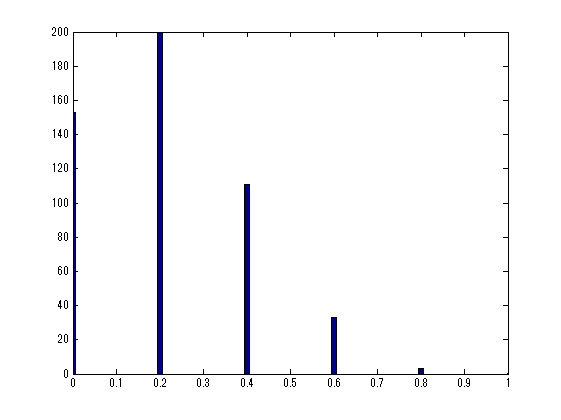
\includegraphics[width=0.5\linewidth]{./kadai/k1/k11.png}
\caption{サイズ5}
\end{figure}

\begin{figure}[htbp]
\centering
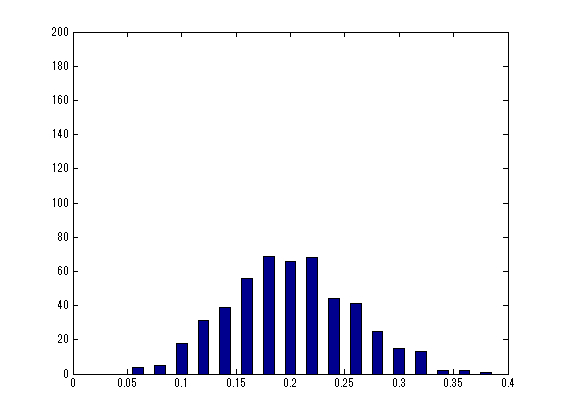
\includegraphics[width=0.5\linewidth]{./kadai/k1/k12.png}
\caption{サイズ50}
\end{figure}

\begin{figure}[htbp]
\centering
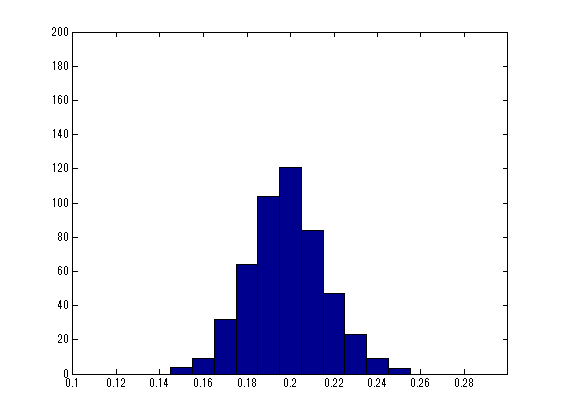
\includegraphics[width=0.5\linewidth]{./kadai/k1/k13.png}
\caption{サイズ500}
\end{figure}

\begin{figure}[htbp]
\centering
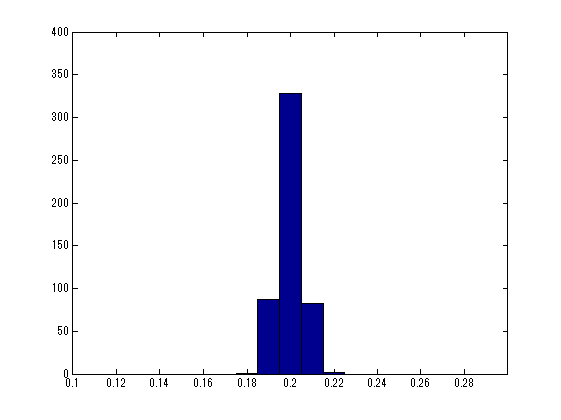
\includegraphics[width=0.5\linewidth]{./kadai/k1/k14.png}
\caption{サイズ5000}
\end{figure}

\newpage\\
\subsection{各々のnについて、 \(N(\mu, \sigma^2/n)\) の確率密度関数のグラフを作成せよ}
\label{sec:org88958d4}
\begin{figure}[htbp]
\centering
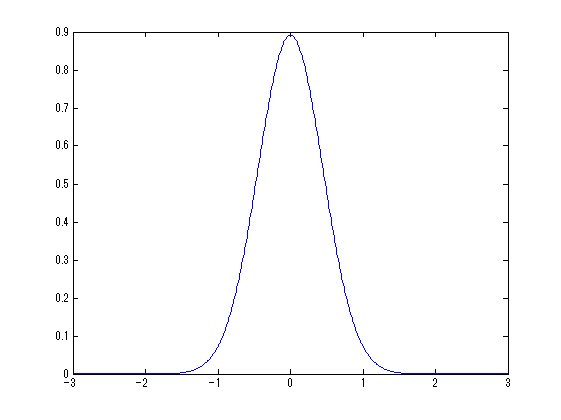
\includegraphics[width=0.5\linewidth]{./kadai/k1/k121.png}
\caption{サイズ5}
\end{figure}

\begin{figure}[htbp]
\centering
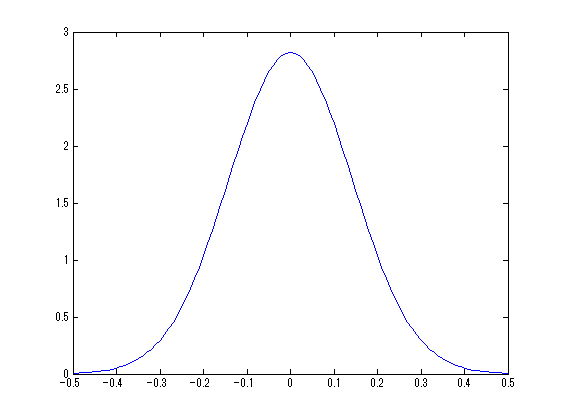
\includegraphics[width=0.5\linewidth]{./kadai/k1/k122.png}
\caption{サイズ50}
\end{figure}

\begin{figure}[htbp]
\centering
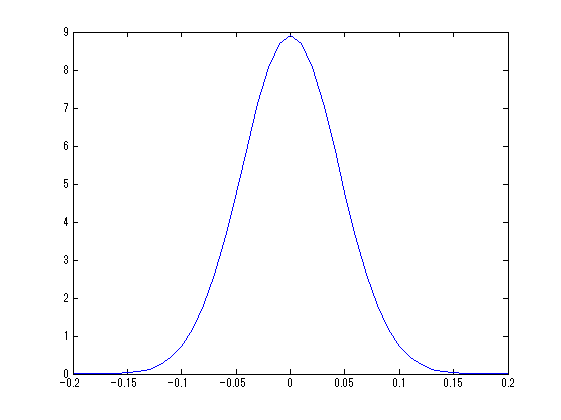
\includegraphics[width=0.5\linewidth]{./kadai/k1/k123.png}
\caption{サイズ500}
\end{figure}

\begin{figure}[htbp]
\centering
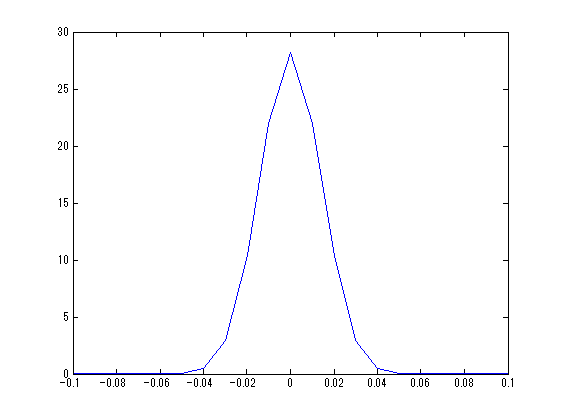
\includegraphics[width=0.5\linewidth]{./kadai/k1/k124.png}
\caption{サイズ5000}
\end{figure}

\newpage\\
\subsection{上の結果を比較して、どのようなことがいえるか、nが小さいときと大きいときとでどのような違いがあるかに注意しながら議論せよ}
\label{sec:org84aedd3}
まず1つ目の問いからは、サイズが増えるごとにそのグラフから正規分布のグラフ形状取りながら分散が小さくなっていることがわかる。2つ目の問いからも同様に確率密度関数が尖ってきていることがわかる。\\
 2つの問いからこのままサンプルのサイズが大きくなるにつれて分散が小さくなり、山の形が尖っていくことが予測できる。\\

\newpage\\
\section{課題2:大数の強法則}
\label{sec:org51f9d16}
\subsection{\(\overline{X}\) の期待値を示せ。また、nが100のとき、20,000のとき、2,000,000の、 \(\overline{X}\) の分散を手計算で求めよ}
\label{sec:orgc190c0f}
\begin{itemize}
\item \(\overline{X}\) の期待値\\
\(E[\overline{X}]
     = E[1/n{\Sigma^{n}_{i=1}{X_k}}] \\
     = 1/n {\Sigma^{n}_{k-1}E[X_k]} \\
     = 1/n {\Sigma^{n}_{k-1}p}\\
     = 1/n (n p) \\
     = p \\
     \because
     E[X_k]
     = \Sigma_{k=0}^{1}kP\{X_k\} \\ 
     = 0 * (1-p) + 1 * p \\
     = p\)\\
\item \(n = 100\) のときの分散\\
\(p(1-p)/n
     = 0.4(1-0.4)/100 \\
     = 0.24/100 \\
     = 0.0024\)\\
\item \(n = 20,000\) のときの分散\\
\(p(1-p)/n
     = 0.4(1-0.4)/20000 \\
     = 0.24/20000 \\
     = 0.000012\)     \\
\item \(n = 20,000,000\) のときの分散\\
\(p(1-p)/n
     = 0.4(1-0.4)/20000000 \\
     = 0.24/20000000 \\
     = 0.000000012\)          \\
\end{itemize}
\subsection{nを増やしていったときの、標本平均の変化を線グラフで表現してみよう}
\label{sec:org8b607b4}
\begin{figure}[htbp]
\centering
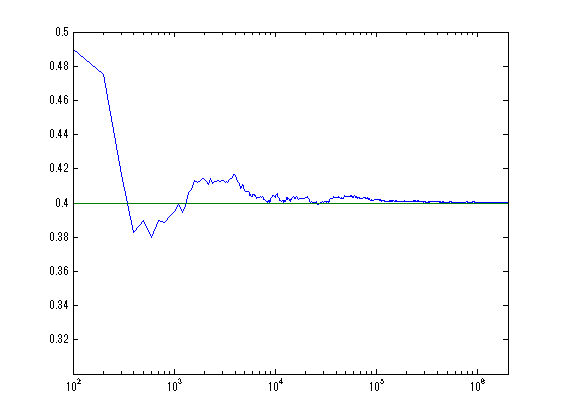
\includegraphics[width=0.5\linewidth]{./kadai/k2/k22.png}
\caption{標本平均の変化}
\end{figure}

\newpage\\
\subsection{上の実験を数回繰り返し、それぞれの結果がどのような点で共通性があるかを確認すること}
\label{sec:org36f50cb}
\begin{figure}[htbp]
\centering
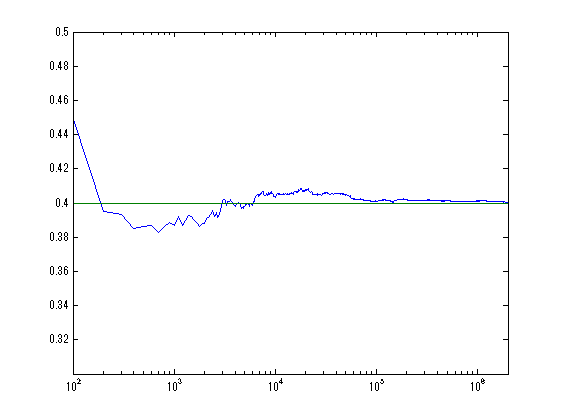
\includegraphics[width=0.5\linewidth]{./kadai/k2/k221.png}
\caption{標本平均の変化-1}
\end{figure}

\begin{figure}[htbp]
\centering
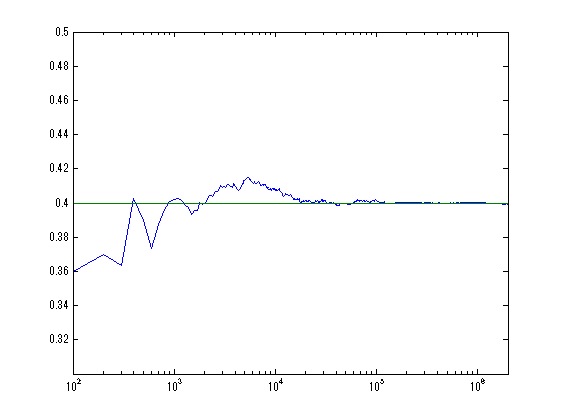
\includegraphics[width=0.5\linewidth]{./kadai/k2/k222.png}
\caption{標本平均の変化-2}
\end{figure}

\begin{figure}[htbp]
\centering
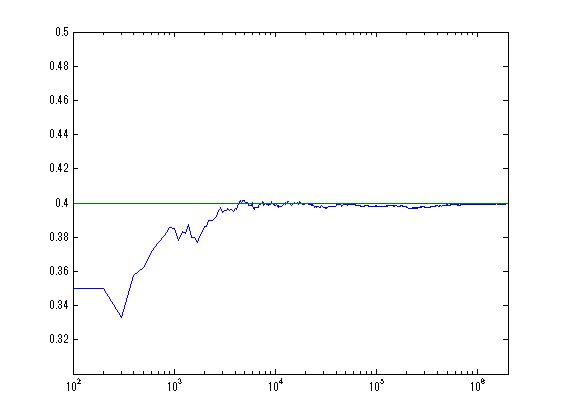
\includegraphics[width=0.5\linewidth]{./kadai/k2/k223.png}
\caption{標本平均の変化-3}
\end{figure}

\begin{figure}[htbp]
\centering
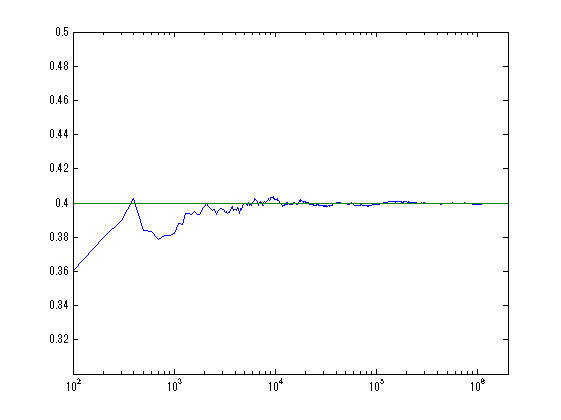
\includegraphics[width=0.5\linewidth]{./kadai/k2/k224.png}
\caption{標本平均の変化-4}
\end{figure}

\begin{figure}[htbp]
\centering
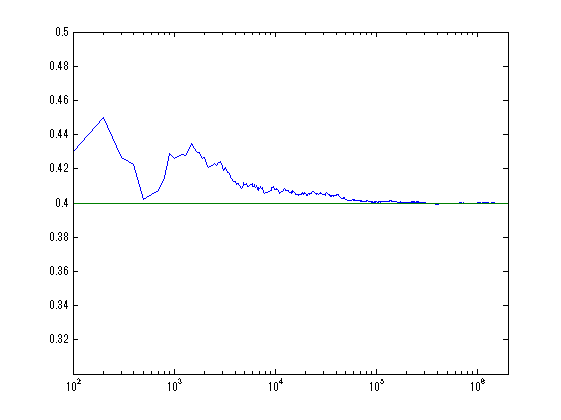
\includegraphics[width=0.5\linewidth]{./kadai/k2/k225.png}
\caption{標本平均の変化-5}
\end{figure}

\newpage   \\
上のグラフで共通する点は、どれもある値 (\(p = 0.4\))で収束していることだ。\\
\subsection{以上の結果から、何が言えるか。}
\label{sec:org4542075}
サンプル数 n が十分に大きいならば、必ずその標本平均が真の平均に近づくという大数の強法則が成り立っていると言える。\\
\end{document}
